\documentclass[tikz,border=10pt]{standalone}
\usepackage{tikz-3dplot}
\usepackage{amsmath, amssymb}
\usetikzlibrary{arrows.meta, positioning, calc, decorations.pathreplacing, 3d}
\usetikzlibrary{matrix, fit, backgrounds, shapes}
\usetikzlibrary{angles,quotes}

\usepackage[T1]{fontenc}
\usepackage[utf8]{inputenc}
\usepackage{newpxtext,newpxmath}
\usepackage{sectsty}

\begin{document}
%========================================================
% TikZ #3 (Step 3): decompose p = alpha u + beta v
%========================================================
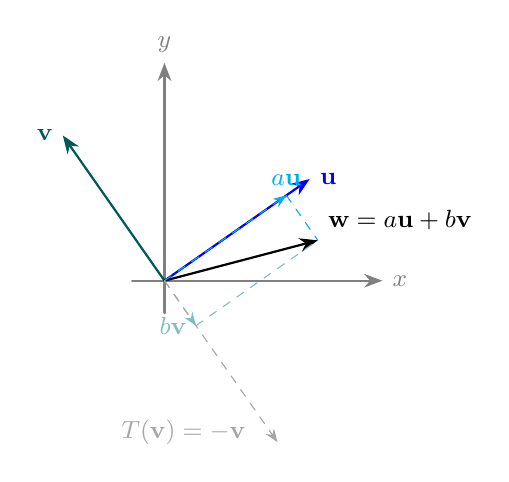
\begin{tikzpicture}[scale=2.05, >=Stealth, line cap=round, line join=round]
	
	\def\m{0.7}
	\def\px{0.95}
	\def\py{0.25}
	
	\pgfmathsetmacro{\ux}{1}
	\pgfmathsetmacro{\uy}{\m}
	\pgfmathsetmacro{\vxB}{-\m}
	\pgfmathsetmacro{\vyB}{1}
	
	\pgfmathsetmacro{\den}{1+(\m)^2}
	\pgfmathsetmacro{\alpha}{(\px + \m*\py)/\den}
	\pgfmathsetmacro{\beta}{(-\m*\px + \py)/\den}
	
	\coordinate (AU)  at ({\alpha*\ux},{\alpha*\uy});
	\coordinate (BV)  at ({\beta*\vxB},{\beta*\vyB});
	\coordinate (SUM) at ({\alpha*\ux+\beta*\vxB},{\alpha*\uy+\beta*\vyB});
	\coordinate (P)   at (\px,\py);
	
	\tikzset{
		axis/.style={thick, gray},
		uvec/.style={thick, blue},
		vvec/.style={thick, teal!70!black},
		pvec/.style={thick, black},
		help/.style={dashed, gray!70},
		box/.style={rounded corners, draw=gray!60, fill=white, inner sep=3pt},
		mat/.style={font=\small}
	}
	
	\newcommand{\panelaxes}{
		\draw[axis,->] (-0.2,0) -- (1.35,0) node[right] {\small $x$};
		\draw[axis,->] (0,-0.2) -- (0,1.35) node[above] {\small $y$};
	}
	
%	\node[box, anchor=west] at (-0.2,1.38) {\small Step 3: write $p=\alpha u+\beta v$};
	
	\panelaxes
	
	\draw[uvec,->] (0,0) -- ({0.9*\ux},{0.9*\uy}) node[pos=1, right] {\small $\textbf{u}$};
	\draw[vvec,->] (0,0) -- ({0.9*\vxB},{0.9*\vyB}) node[pos=1, left]  {\small $\textbf{v}$};
	
	\draw[pvec,->] (0,0) -- (P) node[pos=1, above right] {\small $\textbf{w}=a\textbf{u}+b\textbf{v}$};
	
	\draw[help,->, cyan] (0,0) -- (AU) node[pos=1, above] {\small $a \textbf{u}$};
	\draw[help,->, teal!50] (0,0) -- (BV) node[pos=1, left] {\small $b \textbf{v}$};
	\draw[help,cyan] (AU) -- (SUM);
	\draw[help,teal!50] (BV) -- (SUM);	
	
	\draw[help,->] (0,0) -- ({-\vxB},{-\vyB}) node[pos=0.80, below left] {\small $T(\textbf{v})=-\textbf{v}$};
	
%	\node[anchor=west, mat] at (-0.18,1.05) {$
%		\alpha=\frac{p_x+m p_y}{1+m^2},\quad
%		\beta=\frac{-m p_x+p_y}{1+m^2}$};
	
\end{tikzpicture}	
\end{document}